Preprocessing is a crucial step in the analysis, particularly when the goal is to capture seasonal patterns in the data. To reliably observe seasonality, each time series must cover at least one full yearly cycle. Shorter time series may not contain enough information to capture these effects.

\begin{figure}[h]
    \centering
    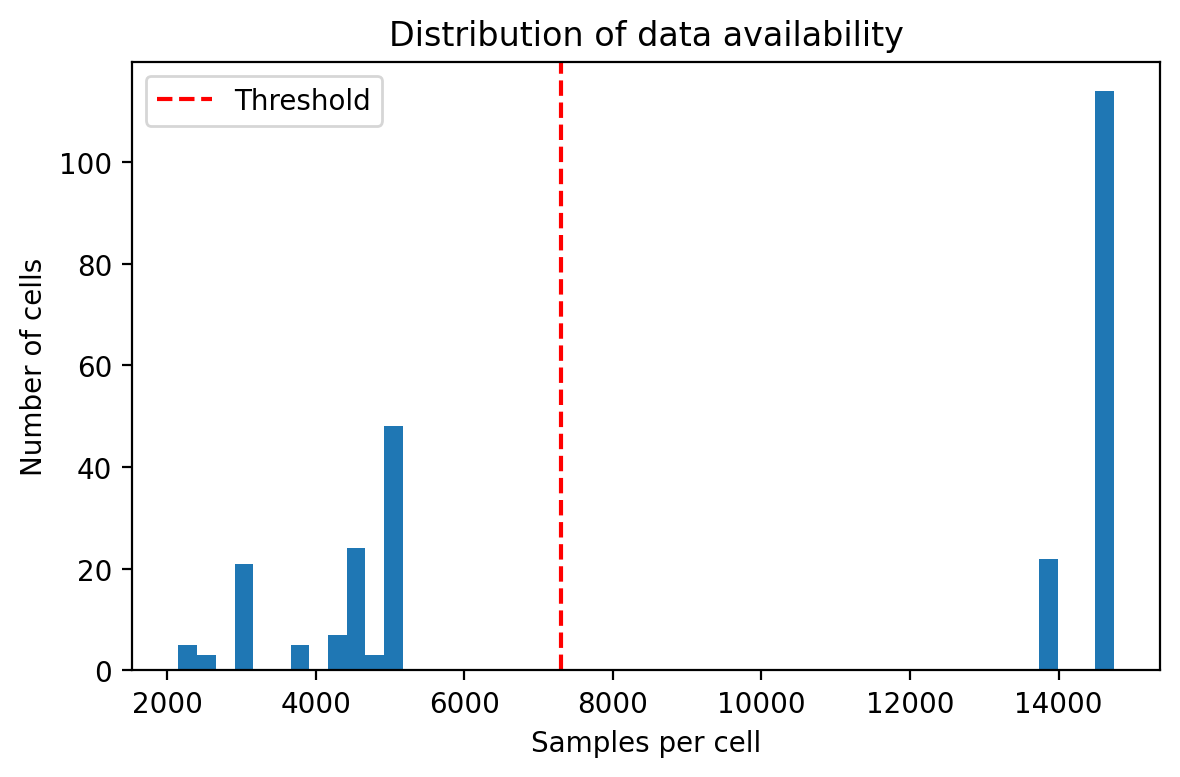
\includegraphics[width=\linewidth]{figures/cell_data_length.png}
    \caption{Distribution of available data samples per cell}
    \label{fig:cell_data_length}
\end{figure}

Figure~\ref{fig:cell_data_length} shows the distribution of the number of observations per cell. Two distinct groups can be observed. The first group contains cells with approximately 15.000 samples, corresponding to more than one year of data. The second group contains cells with roughly 2000-5000 samples, which is below one year of observations. \\

This resulted in the removal of 125 cells due to insufficient length. The removals were distributed across site types as follows: Urban (44), Suburban (48), Recreational (33). \\

%2 Datasets were given as a part of this thesis, 1 with raw KPI's directly from the PM and later on information about the cell such as technology, frequency spectrum. Several cells were missing from the information dataset and such those cells were removed in the process. This included 29 cells, 8 urban, 12 suburban and 9 recreational. Removal of these cells for lacking information about technology and frequency spectrum was certainly not justified, it had gone under my noise and reverse engeneering the technology would not have been an issue

Two datasets were provided as part of this thesis, one containing raw KPIs directly from the PM counters, and a second containing cell-level metadata, including technology generation and frequency spectrum. During preprocessing, cells present in the KPI dataset but missing from the metadata dataset were dropped as part of 
the merge step. This affected 29 cells in total: 8 urban, 12 suburban, and 9 recreational. \\


Duplicate entries at the (site, cell, datetime) level were removed. When duplicates contained conflicting values, rows with non-missing values in the ps data volume dl column were prioritized. This resulted in a deletion of 1,130,288 rows and the dataset going from 3,104,976 to 1,974,688 rows. \\ 


\begin{table}[h]
\centering
\caption{Dataset after preprocessing}
\begin{tabular}{lc}
\hline
\textbf{Statistic} & \textbf{After} \\
\hline
Rows & 1,770,806 \\
Urban sites (cells) & 4 (52) \\
Suburban sites (cells) & 4 (45) \\
Recreational sites (cells) & 4 (39) \\
Cells total & 136 \\
Missing rate (data volume dl) & 166 (0.01\%) \\
Start date & 2024-05-21 \\
End date & 2026-03-01 \\
\hline
\end{tabular}
\end{table}

\subsubsection{Z-score normalization}

Since the analysis focuses on patterns across cells rather than absolute values, Z-score normalization is applied to each cell individually. This transformation ensures that each time series has a mean of 0 and a standard deviation of 1. \\

\begin{equation}
z = \frac{x - \mu}{\sigma}
\end{equation}

Here, $\mu$ is the mean and $\sigma$ is the standard deviation of the values within each cell. \\

By applying this normalization, differences in scale between cells are removed, allowing for direct comparison of patterns in traffic load rather than magnitude differences. \\
